% TeX
%%%%%%%%%%%%%%%%%%%%
% part II of AES2012
\chapter{The Algorithm}
%
\section{The Overview of BSBL Framework}
A block sparse signal $\ve{x}\in\mathbb{C}^{N\times1}$ has the following structure:
\begin{equation}
\ve{x} = [\underbrace{x_1,\cdots,x_{d_1}}_{\ve{x}_1^H},\cdots,
\underbrace{x_1,\cdots,x_{d_g}}_{\ve{x}_g^H}]^H,
\end{equation}
which means $\ve{x}$ has $g$ blocks, and only a few blocks are nonzero. Here $d_i$ is the block size for the $i$th block. To model the intra-block correlation in the $i$-th block, the BSBL framework suggests to use the parameterized Gaussian distribution:
\begin{equation}\label{eq:x_model}
p(\ve{x}_i;{\gamma_i},\ve{B}_i) =
\mathcal{CN}(\ve{x}_i;\mathbf{0},{\gamma_i}\ve{B}_i). 
\end{equation}
with unknown deterministic parameters $\gamma_i$ ($\bm{\gamma}\succeq0$) and $\ve{B}_i$. 

The observation $\ve{y}\in\mathbb{C}^{M\times1}$ is obtained by
\begin{equation}
\ve{y} = \bm{\Phi}\ve{x} + \ve{n},
\end{equation}
where $\bm{\Phi}$ is the sensing matrix and $\ve{n}$ is the observation noise.
The observation noise is assumed to be independent and Complex Gaussian with zero 
mean and variance equal to $\beta^{-1}\ve{I}$. $\beta$ is also unknown. Thus the likelihood is given by
\begin{equation}\label{eq:y_model}
p(\ve{y}|\ve{x};\beta) = \mathcal{CN}(\ve{y};\bm{\Phi}\ve{x},\beta^{-1}\ve{I}). 
\end{equation}

The hierarchical Bayesian model can be illustrated using a probabilistic graph, 
see fig \ref{fig:bm}.
\begin{figure}[!htbp]
\centering
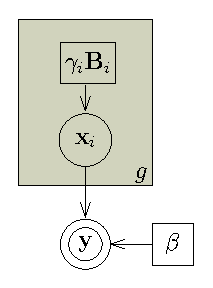
\includegraphics[width=1.2in]{blockmodel}
\caption{The block structural model. The variable $\ve{y}$ in the double 
circled is denoted as observations. The $\ve{x}_i$ in the single circled 
is variables while the value $\gamma_i\ve{B}_i$ and $\beta$ in square box 
are parameters. Shaded box means that each prior $\gamma_i\ve{B}_i$ 
is employed on $\ve{x}_i$ for the range $i\in[1,\cdots,g]$.%
}\label{fig:bm}
\end{figure}
During the learning procedure most $\gamma_i$ tend to be zero, due to the mechanism of automatic relevance determination\cite{Tipping2001}. Thus sparsity in the block level is encouraged\cite{Zhang2011}. $\ve{B}_i\in\mathbb{C}^{d_i\times d_i}$ is a positive definite matrix capturing the correlation structure of the $i$-th block. Although blocks have intra-block correlation, the framework assumes that blocks are mutually independent. 

The posterior $p(\ve{x}|\ve{y}; \{\gamma_i,\ve{B}_i\}_i,\beta)$ and 
the likelihood $p(\ve{y}|\{\gamma_i,\ve{B}_i\}_i,\beta)$ can be calculated as
\begin{equation}
p(\ve{x}|\ve{y}; \{\gamma_i,\ve{B}_i\}_i,\beta) = 
\frac{p(\ve{x}_i;{\gamma_i},\ve{B}_i)p(\ve{y}|\ve{x};\beta)}{p(\ve{y}|\{\gamma_i,\ve{B}_i\}_i,\beta)},
\end{equation}
given the data model \eqref{eq:x_model} and the observation model \eqref{eq:y_model},
we apply the Gaussian Identity\cite{Petersen2008},
\begin{align}
p(\ve{x}|\ve{y}; \{\gamma_i,\mathbf{B}_i\}_i,\beta) &=
\mathcal{CN}(\ve{x};\bm{\mu},\bm{\Sigma}), \\
p(\ve{y}|\{\gamma_i,\ve{B}_i\}_i,\beta) &= 
\mathcal{CN}(\ve{y};\ve{0},\ve{C}),
\end{align}
where
$\bm{\Sigma} \triangleq (\bm{\Gamma}^{-1} + \bm{\Phi}^H\beta\bm{\Phi})^{-1}$,
$\bm{\mu} \triangleq \bm{\Sigma}\bm{\Phi}^H\beta\ve{y}$ and
$\ve{C} \triangleq \beta^{-1}\ve{I} + \bm{\Phi}\bm{\Gamma}\bm{\Phi}^H$ where
$\bm{\Gamma}$ denotes a block diagonal matrix with the $i$th principal block
given by $\gamma_i\ve{B}_i$.

Once all the parameters, namely $\{\gamma_i,\mathbf{B}_i\}_i,\beta$,  are estimated, the MAP estimate of the signal $\mathbf{x}$ can be directly obtained from the mean of the posterior, i.e.,
\begin{equation}
\mathbf{x} = \bm{\Sigma}\bm{\Phi}^H\beta\ve{y}. \label{eq:Rule_x}
\end{equation}

To estimate the parameters,  the following cost function is generally used, which is derived from the Type II maximum likelihood \cite{Zhang2012a}:
\begin{align}
\mathcal{L}(\{\gamma_i,\mathbf{B}_i\}_i,\beta)
 &= \log\abs{\ve{C}} + \ve{y}^H\ve{C}^{-1}\ve{y}, \label{eq:loglikelihood}
\end{align}
There are several methods to minimize the cost function \cite{Zhang2012a}. In the following we consider to use the marginalized likelihood maximization method, which was used by Tipping et al. \cite{Faul2002} for their basic SBL algorithm and later was used by Ji et al. \cite{Ji2008} for their Bayesian compressive sensing algorithm.

%%%%
\section{The Proposed Block SBL Algorithm}

\subsection{The Mainbody of the Algorithm}
The cost function \eqref{eq:loglikelihood} can be optimized in a block way.
We denote by $\bm{\Phi}_i$
the $i$th block in $\bm{\Phi}$ with the column indexes  corresponding to
the $i$th block
of the signal $\ve{x}$. Then $\ve{C}$ can be rewritten as:
\begin{align}
\ve{C} &= \beta^{-1}\ve{I} + \sum_{m\neq i} \bm{\Phi}_m\gamma_m\ve{B}_m\bm{\Phi}_m^H+
\bm{\Phi}_i\gamma_i\ve{B}_i\bm{\Phi}_i^H, \\
 &= \ve{C}_{-i} + \bm{\Phi}_i\gamma_i\ve{B}_i\bm{\Phi}_i^H, \label{eq:c}
\end{align}
where $\ve{C}_{-i} \triangleq \beta^{-1}\ve{I} + \sum_{m\neq i} \bm{\Phi}_m\gamma_m\ve{B}_m\bm{\Phi}_m^H$.
Using the Woodbury Identity,
\begin{align}
\abs{\ve{C}} &= \abs{\gamma_i\ve{B}_i}\abs{\ve{C}_{-i}}\abs{\ve{A}_i^{-1} + \ve{s}_i}, \\
\ve{C}^{-1} &= \ve{C}_{-i}^{-1} - \ve{C}_{-i}^{-1}\bm{\Phi}_i(\ve{A}_i^{-1} + \ve{s}_i)^{-1}\bm{\Phi}_i^H\ve{C}_{-i}^{-1},
\end{align}
where $\ve{A}_i\triangleq\gamma_i\ve{B}_i$,
$\ve{s}_i\triangleq \bm{\Phi}_i^H\ve{C}_{-i}^{-1}\bm{\Phi}_i$, and
$\ve{q}_i\triangleq\bm{\Phi}_i^H\ve{C}_{-i}^{-1}\ve{y}$,
the Equation \eqref{eq:loglikelihood} can be rewritten as:
\begin{align}
\mathcal{L} =& \log\abs{\ve{C}_{-i}} + \ve{y}^H\ve{C}_{-i}^{-1}\ve{y} \nonumber \\
 &+ \log\abs{\ve{I}_{d_i} + \ve{A}_i\ve{s}_i} - \ve{q}_i^H(\ve{A}_i^{-1} + \ve{s}_i)^{-1}\ve{q}_i, \\
 =& \mathcal{L}(-i) + \mathcal{L}(i),
\end{align}
where $\mathcal{L}(-i) \triangleq \log\abs{\ve{C}_{-i}} + \ve{y}^H\ve{C}_{-i}^{-1}\ve{y}$, and
\begin{equation}\label{eq:lgi}
\mathcal{L}(i) =
\log\abs{\ve{I}_{d_i} + \ve{A}_i\ve{s}_i} -
\ve{q}_i^H(\ve{A}_i^{-1} + \ve{s}_i)^{-1}\ve{q}_i,
\end{equation}
which only depends on $\gamma_i$ and $\mathbf{B}_i$.

Setting  $\frac{\partial \mathcal{L}(i)}{\partial \gamma_i} = 0$, we have the updating rule
\begin{equation}\label{eq:gamma_0}
\gamma_i = \frac{1}{d_i}\mathrm{Tr}\left[\ve{B}_i^{-1}\ve{s}_i^{-1}(\ve{q}_i\ve{q}_i^H - \ve{s}_i)\ve{s}_i^{-1}\right].
\end{equation}

Setting $\frac{\partial \mathcal{L}(i)}{\partial \ve{B}_i}=\ve{0}$, we have the updating rule
\begin{equation}\label{eq:b_0}
\ve{B}_i = \frac{\ve{s}_i^{-1}(\ve{q}_i\ve{q}_i^H - \ve{s}_i)\ve{s}_i^{-1}}
{\gamma_i}.
\end{equation}

%The derivation of \eqref{eq:gamma_0} and \eqref{eq:b_0} is given in the Appendix \ref{app:update_formula}.

{\bf Remark~I:} The update equation \eqref{eq:gamma_0} for $\gamma_i$ guarrantted that $\gamma_i\in\mathbb{R}$. The matrix $\ve{C}$ (see eq\eqref{eq:c}) is a Hermite matrix with that $\ve{C}^H=\ve{C}$, and consequently $\ve{s}_i=\bm{\Phi}_i^H\ve{C}_{-i}^{-1}\bm{\Phi}_i$ is also a Hermite matrix. We let $\ve{a}=\mathrm{diag}[\ve{s}_i^{-1}(\ve{q}_i\ve{q}_i^H - \ve{s}_i)\ve{s}_i^{-1}]$, and the following property holds: $\ve{a}\in\mathbb{R}^{d_i\times1}$ and $\gamma_i=\mathrm{mean}(\ve{a})$.

{\bf Remark~II:} The algorithm start with $\ve{B}_i=\ve{I}_{d_i}, \forall i$, iteratively update $\gamma_i$ using \eqref{eq:gamma_0} and then calculating the intra-correlation $\ve{B}_i$ using \eqref{eq:b_0}.

\subsection{The Stationary Point of Block SBL}
The stationary solution of block BCS can be analyzed by inspecting the second partial 
derivation (see \cite{Faul2002,Tipping2003}) of \eqref{eq:lgi}. 
In the Fast Marginalized Block SBL algorithm, the analysis of the stationary point 
is put in the Appendix %\ref{app:stationary_point}
for not affecting the reader. We only give the 
simple conclusion in this section.

%For a given block basis $i$, the update schema for $\gamma_i$ is:
%\begin{enumerate}
%\item when $\rho_i<0$. The solution in \eqref{eq:lgi_1st_order} is negative, 
%and since $\partial\mathcal{L}(\gamma_i)/\partial\gamma_i|_{\gamma_i=0}>0$, 
%the minimization occurs at $\gamma_i=0$;
%\item when $\rho_i>0$. The solution in \eqref{eq:lgi_1st_order} is positive. 
%We have $\partial\mathcal{L}(\gamma_i)/\partial\gamma_i|_{\gamma_i=0}<0$ and 
%$\partial\mathcal{L}(\gamma_i)/\partial\gamma_i|_{\gamma_i=\infty}>0$, the 
%obtained value of $\gamma_i$ thus minimize $\mathcal{L}(\gamma_i)$;
%\item when $\rho_i=0$. The solution in \eqref{eq:lgi_1st_order} is equal to 0, 
%the relevant basis can be pruned out from the model.
%\end{enumerate}

The minimization of $\mathcal{L}(\bm{\gamma})$ can be iteratively 
updated using,
\begin{equation}\label{eq:lgi_solution}
\tilde\gamma_i = \left\{
\begin{aligned}
\gamma_i,\quad & \gamma_i>0 \\
0,\quad &\gamma_i\leq0
\end{aligned} \right. ,
\end{equation}
where $\gamma_i$ is calculated using \eqref{eq:gamma_0} and 
$\tilde{\gamma}_i$ denotes the updated value of $\gamma_i$.

\subsection{The Change of The Log-Likelihood of Fast Marginalized block SBL}
By calculating all $\rho_i$, the potential operation on the basis is illustrated in 
fig \ref{fig:basis_select}.
\begin{figure}[!htbp]
\centering
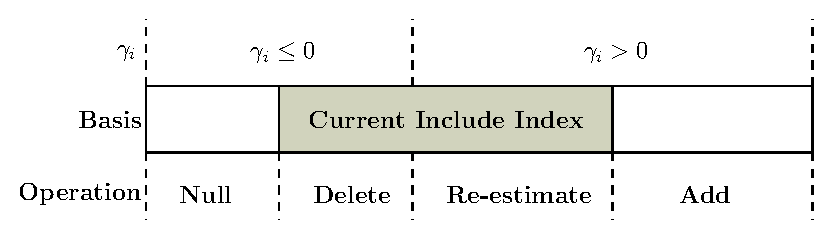
\includegraphics[width=3.3in]{basis_select}
\caption{The operation on the basis w.r.t $\gamma_i$. 
The currently included block basis at iteration $k$ is denoted as the shaded area.
Those indices correspond to $\gamma_i\leq0$ will be pruned out at iteration $k+1$ while
the one with $\gamma_i>0$ will be add in or re-estimated.
}\label{fig:basis_select}
\end{figure}
The change of the log-likelihood (see eq \eqref{eq:lgi}) is calculated as:
\begin{equation}
\Delta \mathcal{L}(\gamma_i) = \mathcal{L}(\tilde{\gamma_i}) - \mathcal{L}(\gamma_i).
\end{equation}
By calculating $\Delta\mathcal{L}(\gamma_i),\forall i$, 
the minimal value of $\Delta \mathcal{L}(\gamma_i)$ and the correspond basis
is selected to boost the convergence speed in saughting the minimum of 
the cost function $\mathcal{L}(\bm{\gamma})$.

\subsection{Remarks on $\beta$}

The parameter $\beta^{-1}$ is the noise variance in our model. It can be estimated by a number of methods.  However, the resulting updating rule is generally not robust and requires some regularization \cite{Zhang2012a,Zhang2011}. In practice, people treat it as a regularizer and assign some specific values to it \footnote{For example, one can see this by examining the published codes of the algorithms in \cite{Ji2008,Babacan2012}.}. Similar to \cite{Ji2008},
we select $\beta=10^{-6}$ in noiseless simulations, $\beta=0.1\norm{y}_2^2$ in general noisy scenarios (e.g. $\text{SNR}<20$ dB), and $\beta=0.01\norm{y}_2^2$ in high SNR scenarios (e.g. $\text{SNR}\geq20$ dB).

\subsection{The Fast Marginalized block SBL Algorithm}
%%
The Fast Marginalized block SBL algorithm ({\bf BSBL-FM})
is given in Fig. \ref{algo:bsbl-fm},
In the remaining of this paper, we denote
{\bf BSBL-FM(0)} as the algorithm ignores the intra-block correlation (i.e.
$\ve{B}_i=\ve{I}_{d_i}$), {\bf BSBL-FM(1)} as the one iteratively update 
the intra-block correlation $\ve{B}_i$.
%The updates formulas of
%$\bm{\mu}$, $\bm{\Sigma}$, $\ve{s}$ and $\ve{q}$ are given in the 
%Appendix \ref{app:update_quantities}.

\begin{algorithm}[!htb]
\caption{The BSBL-FM Algorithm.}\label{algo:bsbl-fm}
\begin{algorithmic}[1]
\STATE outputs: $\ve{w},\bm{\Sigma},\bm{\gamma}$.
\WHILE{convergence criterion not met}
\STATE Calculate $\gamma_i$, $\ve{B}$ using \eqref{eq:gamma_0} and \eqref{eq:b_0};
\STATE Calculate $\Delta \mathcal{L}(\gamma_i)$;
\STATE Select block $i$ with $\Delta\mathcal{L}(\gamma_i)=\min\Delta\mathcal{L}(\gamma_i)$;
\IF{add}
\STATE Process {\bf add} on quantities $\bm{\mu},\bm{\Sigma},\ve{s},\ve{q}$.
\ELSIF{re-estimate}
\STATE Process {\bf re-estimate} on $\bm{\mu},\bm{\Sigma},\ve{s},\ve{q}$.
\ELSIF{delete}
\STATE Process {\bf delete} on quantities $\bm{\mu},\bm{\Sigma},\ve{s},\ve{q}$.
\ENDIF
\STATE Re-calculate the convergence criterion.
\ENDWHILE
\end{algorithmic}
\end{algorithm}

\section{Reformulated ARD and Incremental Block ARD Schemes}
The objective function $\mathcal{L}(\bm{\gamma})$ can be up bounded as
\begin{equation}
\mathcal{L}(\ve{z},\bm{\gamma}) = \ve{z}^T\bm{\gamma} - h^*(\ve{z}) + \ve{y}^T\ve{C}^{-1}\ve{y},
\end{equation}
where $\ve{z}=[\ve{z}_1,\cdots,\ve{z}_g]^T$ and $h^*(\ve{z})$ is the concave conjugate of 
$\log\abs{\ve{C}}$ defined by the duality relationship 
$h^*(\ve{z})=\min_{\bm{\gamma}}\ve{z}^T\bm{\gamma} - \log\abs{\ve{C}}$.
Then for $\bm{\gamma}$ fixed at $\hat{\bm{\gamma}}$, the tightest upper bound of 
$\mathcal{\bm{\gamma}}$ is obtained by minimizing 
$\mathcal{L}(\bm{\gamma},\ve{z})|_{\bm{\gamma}=\hat{\bm{\gamma}}}=\mathcal{L}(\ve{z};\hat{\bm{\gamma}})$
over all $\ve{z}$, the corresponding minimizer can be found in closed form:
\begin{equation}
\ve{z} = \mathrm{diag}(\bm{\Phi}^T\ve{C}^{-1}\bm{\Phi}),
\end{equation}
now be fix $\ve{z}$ at $\hat{\ve{z}}$, the $\mathcal{L}(\bm{\gamma};\hat{\ve{z}})$ is minimized 
by solving 
\begin{equation}
\bm{\gamma} = \arg\min_{\bm{\gamma}} \hat{\ve{z}}^T\bm{\gamma} + \ve{y}^T\ve{C}^{-1}\ve{y},
\end{equation}
which again can be partitioned as,
\begin{align}
\mathcal{L}(\bm{\gamma};\hat{\ve{z}}) =& \sum_{k\neq i}\ve{z}_k^T\bm{\gamma}_k + \ve{y}^T\ve{C}_{-i}^{-1}\ve{y} \\
& +\ve{z}_i^T\bm{\gamma}_i - \ve{q}_i^T(\ve{A}_i^{-1} + \ve{s}_i)^{-1}\ve{q}_i,
\end{align}

\section{Structured Regularized Block-SBL Method}
{\bf biblio blaze: structured matrices, Geometric methods for estimation of 
structured covariances, structure regularized learning, }

\subsection{Regularization to $\mathbf{B}_i$}

As noted in \cite{Zhang2012a},  regularization to $\mathbf{B}_i$ is required due to limited data. It has been shown \cite{Zhang2011} that in noiseless cases the regularization does not affect the global minimum of the cost function (\ref{eq:loglikelihood}), i.e., the global minimum still corresponds to the true solution; the regularization only affects the probability of the algorithm to converge to the local minima. A good regularization can largely reduce the probability of local convergence. Although theories on regularization strategies are lacked, some empirical methods \cite{Zhang2011,Zhang2012a} were presented in literature.

It should be noted that the information of the signal structure within each block
can be well described by the covariance matrices $\ve{B}_i$.
Exploiting such information can potentially improve the recovery performance.
In the following, we firstly adopting the empirical approximation method 
proposed in \cite{Zhang2012a}; and then proposed a geometric methods for
estimating the underlying Toeplitz matrix.

\subsection{Regularized using AR(1) Model\cite{Zhang2012}}
Our algorithm can conveniently utilizing the regularization used in \cite{Zhang2012a},
which model the entries in each block as a first-order Auto-Regressive (AR) process with the AR coefficient $r_i$. As a result,
$\ve{B}_i$ has the following form
\begin{equation}
\ve{B}_i = \mathrm{Toeplitz}([1,r_i,\cdots,r_i^{d_i-1}]). \label{equ:Bi}
\end{equation}
where $\mathrm{Toeplitz}(\cdot)$ is a Matlab command expanding a real vector into a
symmetric Toeplitz matrix. Thus the correlation level of the intra-block correlation is reflected by the value of $r_i$. $r_i$ can be estimated from the cost function (\ref{eq:loglikelihood}) directly, or can be empirically roughly calculated from the estimated $\ve{B}_i$ in (\ref{eq:b_0}) as shown in \cite{Zhang2012a}. We used the latter method, since it provides satisfactory results and saves lots of computation. According to \cite{Zhang2012a}, $r_i$ is calculated by $r_i \triangleq\frac{m_1^i}{m_0^i}$,
where $m_0^i$ (res. $m_1^i$) is the average of entries along the main diagonal
(res. the main sub-diagonal) of the matrix $\ve{B}_i$. This calculation cannot ensure $r_i$ has a feasible value, i.e. $|r_i|<0.99$.
Thus in practice, we calculate $r_i$ by
\footnote{%
this constrain guaranteed that the determinant of $\ve{B}_i$, 
which is $(1-r_i^2)^{d_i-1}$, is positive} %
\begin{align}
r_i &= \mathrm{sign}(\frac{m^i_1}{m^i_0}) \min \Big\{\Big|\frac{m^i_1}{m^i_0}\Big|,0.99 \Big\}. \label{equ:r_i}
\end{align}
Our algorithm using this regularization (\ref{equ:Bi})-(\ref{equ:r_i}) is denoted by {\bf BSBL-FM(1)}.


In many real-world applications, the intra-block correlation in each block of a signal
tends to be positive and high together. Thus, one can further constrain that
all the intra-block
correlation values of blocks have the same AR coefficient $r$ \cite{Zhang2012a}, where $r$ is the average of all the $r_i$,
\begin{align}
r &= \frac{1}{g}\sum_{i=1}^g r_i.  \label{equ:r}
\end{align}
Then, $\mathbf{B}_i$ is reconstructed as
\begin{eqnarray}
\mathbf{B}_i = \mathrm{Toeplitz}([1,r,\cdots,r^{d_i-1}]). \label{equ:B}
\end{eqnarray}
Our algorithm using this regularization (\ref{equ:r})-(\ref{equ:B}) is denoted by {\bf BSBL-FM(2)}.

\subsection{Regularized using Geometric method with Toeplitz Constrains}
The update equation for $\ve{B}_i$ (see \eqref{eq:b_0}) can not be directly used,
due to the fact that the matrix obtained using \eqref{eq:b_0} may not be toeplitz 
due to statistical errors, and is sometimes badly conditioned,
which will cause numerical errors during the iteration process.

Many other forms of constrains, such as Temporal Smooth Matrix\cite{Chen2007,Zhou2011}
or Band-Toeplitz Matrix can also be used in a similar manner.

%%%%%%%%%%%%%%%%%%%%%%%%%%%%%%%%%%%%%%%%%%%%%%%%%%%%%%%%%%%%%%%%%%%%%%%%%%%%%%%
% Ning2011
We focus on the problem of estimating the Toeplitz covariance from 
finite observations. 
The Toeplitz matrix is sought as the one closest to $\ve{B}_i$ in a 
suitable geometry. 

\subsubsection{Geometry Viewpoint}
Given $\ve{B}_i$, we consider the problem to minimize
\begin{equation}
\min_{\ve{T}\in\mathcal{T}} d(\ve{T},\ve{B}),
\end{equation}
over the class of admissible matrices
\begin{equation}
\mathcal{T} \triangleq \{\ve{T}:\ve{T}\succeq0, \ve{T}~\text{beging Toeplitz}\}.
\end{equation}



